% exemple algorithme de Roy

\begin{frame}{Exemple}
    \begin{center}
        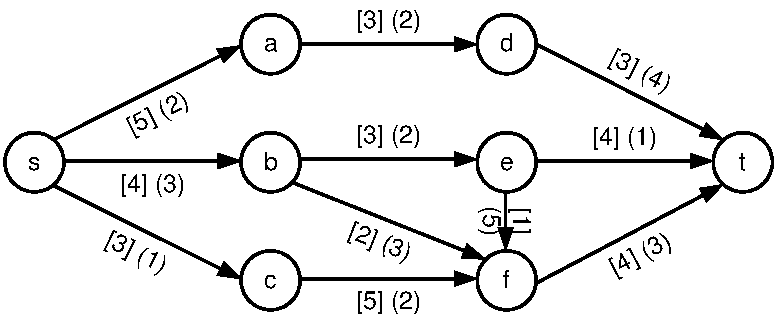
\includegraphics[width=.8\textwidth]{fig/fmcm1.pdf}
    \end{center}
\end{frame}

\begin{frame}{Premier graphe résiduel : le graphe lui-même}
    \begin{center}
        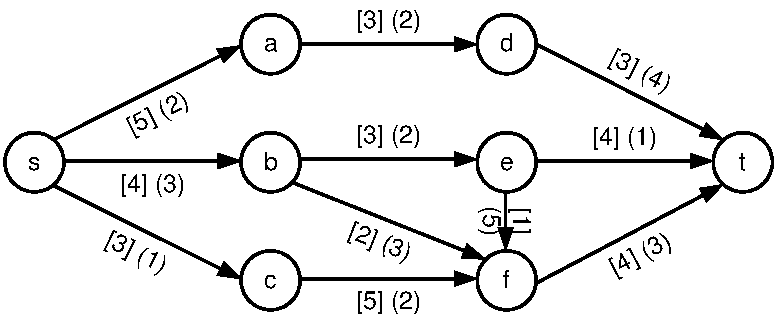
\includegraphics[width=.8\textwidth]{fig/fmcm1.pdf}
    \end{center}

    Plus court chemin : $(s,b,e,t)$ de capacité 3. On augmente le flot de 3.
\end{frame}

\begin{frame}{Second graphe résiduel}
    \begin{center}
        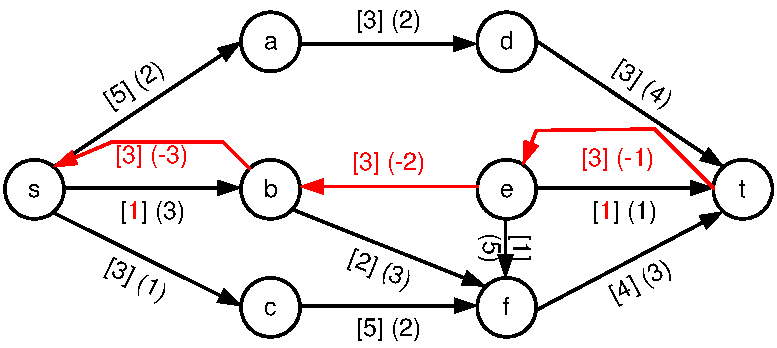
\includegraphics[width=.8\textwidth]{fig/fmcm2.pdf}
    \end{center}

    Plus court chemin : $(s,c,f,t)$ de capacité 3. On augmente le flot de 3.
\end{frame}

\begin{frame}{Troisième graphe résiduel}
    \begin{center}
        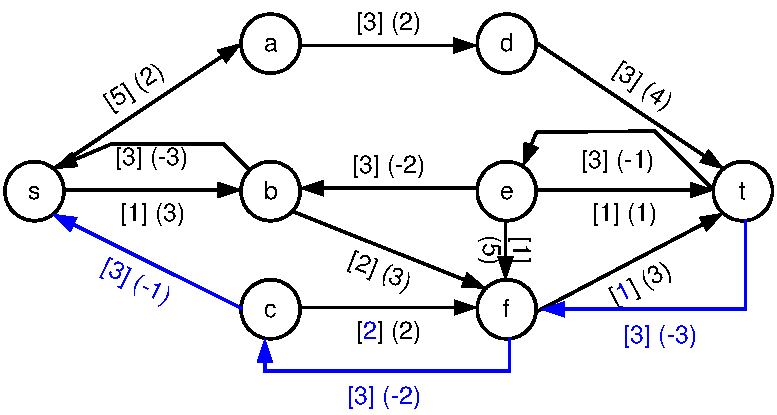
\includegraphics[width=.8\textwidth]{fig/fmcm3.pdf}
    \end{center}

    Plus court chemin : $(s,a,d,t)$ de capacité 3. On augmente le flot de 3.
\end{frame}

\begin{frame}{Quatrième graphe résiduel}
    \begin{center}
        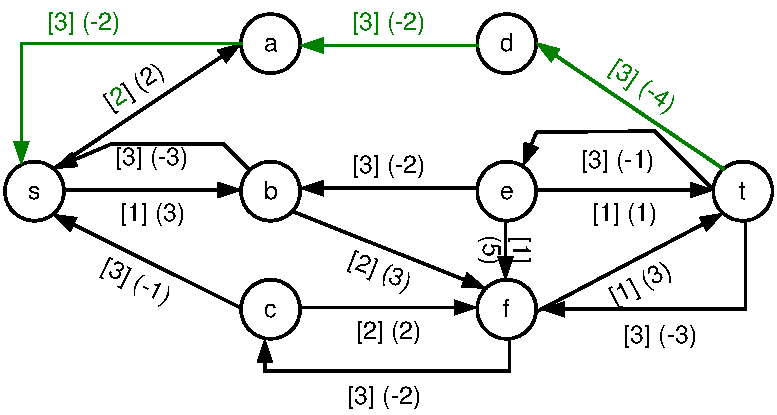
\includegraphics[width=.8\textwidth]{fig/fmcm4.pdf}
    \end{center}

    Plus court chemin : $(s,b,f,t)$ de capacité 1. On augmente le flot de 1.
\end{frame}

\begin{frame}{Cinquième graphe résiduel}
    \begin{center}
        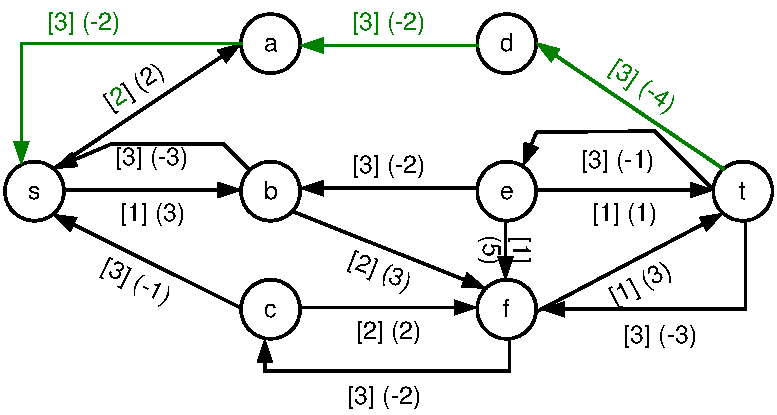
\includegraphics[width=.8\textwidth]{fig/fmcm4.pdf}
    \end{center}

    Pas de chemin entre $s$ et $t$ : l'algorithme est terminé.
\end{frame}



